\message{ !name(isvc_submission.tex)}%last updated in April 2002 by Antje Endemann

\documentclass[runningheads]{llncs}
%In order to omit page numbers and running heads
%please use the following line instead of the first command line:
%\documentclass{llncs}.
%Furthermore change the line \pagestyle{headings} to
%\pagestyle{empty}.

% Psfig/TeX 
\def\PsfigVersion{1.10}
\def\setDriver{\DvipsDriver} % \DvipsDriver or \OzTeXDriver
%
% All software, documentation, and related files in this distribution of
% psfig/tex are Copyright 1993 Trevor J. Darrell
%
% Permission is granted for use and non-profit distribution of psfig/tex 
% providing that this notice is clearly maintained. The right to
% distribute any portion of psfig/tex for profit or as part of any commercial
% product is specifically reserved for the author(s) of that portion.
%
% To use with LaTeX, use \documentstyle[psfig,...]{...}
% To use with TeX, use \input psfig.sty
%
% Bugs and improvements to trevor@media.mit.edu.
%
% Thanks to Ned Batchelder, Greg Hager (GDH), J. Daniel Smith (JDS),
% Tom Rokicki (TR), Robert Russell (RR), George V. Reilly (GVR),
% Ken McGlothlen (KHC), Baron Grey (BG), Gerhard Tobermann (GT).
% and all others who have contributed code and comments to this project!
%
% ======================================================================
% Modification History:
%
%  9 Oct 1990   JDS	used more robust bbox reading code from Tom Rokicki
% 29 Mar 1991   JDS	implemented rotation= option
% 25 Jun 1991   RR	if bb specified on cmd line don't check
%			for .ps file.
%  3 Jul 1991	JDS	check if file already read in once
%  4 Sep 1991	JDS	fixed incorrect computation of rotated
%			bounding box
% 25 Sep 1991	GVR	expanded synopsis of \psfig
% 14 Oct 1991	JDS	\fbox code from LaTeX so \psdraft works with TeX
%			changed \typeout to \ps@typeout
% 17 Oct 1991	JDS	added \psscalefirst and \psrotatefirst
% 23 Jun 1993   KHC     ``doclip'' must appear before ``rotate''
% 27 Oct 1993   TJD	removed printing of filename to avoid 
%			underscore problems. changed \frame to \fbox.
%			Added OzTeX support from BG. Added new
%			figure search path code from GT.
%
% ======================================================================
%
% Command synopsis:
%
% \psdraft	draws an outline box, but doesn't include the figure
%		in the DVI file.  Useful for previewing.
%
% \psfull	includes the figure in the DVI file (default).
%
% \psscalefirst width= or height= specifies the size of the figure
% 		before rotation.
% \psrotatefirst (default) width= or height= specifies the size of the
% 		 figure after rotation.  Asymetric figures will
% 		 appear to shrink.
%
% \psfigurepath{dir:dir:...}  sets the path to search for the figure
%
% \psfig
% usage: \psfig{file=, figure=, height=, width=,
%			bbllx=, bblly=, bburx=, bbury=,
%			rheight=, rwidth=, clip=, angle=, silent=}
%
%	"file" is the filename.  If no path name is specified and the
%		file is not found in the current directory,
%		it will be looked for in directory \psfigurepath.
%	"figure" is a synonym for "file".
%	By default, the width and height of the figure are taken from
%		the BoundingBox of the figure.
%	If "width" is specified, the figure is scaled so that it has
%		the specified width.  Its height changes proportionately.
%	If "height" is specified, the figure is scaled so that it has
%		the specified height.  Its width changes proportionately.
%	If both "width" and "height" are specified, the figure is scaled
%		anamorphically.
%	"bbllx", "bblly", "bburx", and "bbury" control the PostScript
%		BoundingBox.  If these four values are specified
%               *before* the "file" option, the PSFIG will not try to
%               open the PostScript file.
%	"rheight" and "rwidth" are the reserved height and width
%		of the figure, i.e., how big TeX actually thinks
%		the figure is.  They default to "width" and "height".
%	The "clip" option ensures that no portion of the figure will
%		appear outside its BoundingBox.  "clip=" is a switch and
%		takes no value, but the `=' must be present.
%	The "angle" option specifies the angle of rotation (degrees, ccw).
%	The "silent" option makes \psfig work silently.
%
% ======================================================================
% check to see if macros already loaded in (maybe some other file says
% "\input psfig") ...
\ifx\undefined\psfig\else\endinput\fi
%
% from a suggestion by eijkhout@csrd.uiuc.edu to allow
% loading as a style file. Changed to avoid problems
% with amstex per suggestion by jbence@math.ucla.edu

\let\LaTeXAtSign=\@
\let\@=\relax
\edef\psfigRestoreAt{\catcode`\@=\number\catcode`@\relax}
%\edef\psfigRestoreAt{\catcode`@=\number\catcode`@\relax}
\catcode`\@=11\relax
\newwrite\@unused
\def\ps@typeout#1{{\let\protect\string\immediate\write\@unused{#1}}}

\def\DvipsDriver{
	\ps@typeout{psfig/tex \PsfigVersion -dvips}
\def\PsfigSpecials{\DvipsSpecials} 	\def\ps@dir{/}
\def\ps@predir{} }
\def\OzTeXDriver{
	\ps@typeout{psfig/tex \PsfigVersion -oztex}
	\def\PsfigSpecials{\OzTeXSpecials}
	\def\ps@dir{:}
	\def\ps@predir{:}
	\catcode`\^^J=5
}

%% Here's how you define your figure path.  Should be set up with null
%% default and a user useable definition.

\def\figurepath{./:}
\def\psfigurepath#1{\edef\figurepath{#1:}}

%%% inserted for Searching Unixpaths
%%% (the path must end with :)
%%% (call: \DoPaths\figurepath )
%%%------------------------------------------------------
\def\DoPaths#1{\expandafter\EachPath#1\stoplist}
%
\def\leer{}
\def\EachPath#1:#2\stoplist{% #1 part of the list (delimiter :)
  \ExistsFile{#1}{\SearchedFile}
  \ifx#2\leer
  \else
    \expandafter\EachPath#2\stoplist
  \fi}
%
% exists the file (does not work for directories!)
%
\def\ps@dir{/}
\def\ExistsFile#1#2{%
   \openin1=\ps@predir#1\ps@dir#2
   \ifeof1
       \closein1
       %\ps@typeout{...not: \ps@predir#1\ps@dir#2}
   \else
       \closein1
       %\ps@typeout{...in:  \ps@predir#1\ps@dir#2}
        \ifx\ps@founddir\leer
          %\ps@typeout{set founddir #1}
           \edef\ps@founddir{#1}
        \fi
   \fi}
%------------------------------------------------------
%
% Get dir in path or error
%
\def\get@dir#1{%
  \def\ps@founddir{}
  \def\SearchedFile{#1}
  \DoPaths\figurepath
%  \fi
}
%------------------------------------------------------
%%% END of Searching Unixpaths


%
% @psdo control structure -- similar to Latex @for.
% I redefined these with different names so that psfig can
% be used with TeX as well as LaTeX, and so that it will not 
% be vunerable to future changes in LaTeX's internal
% control structure,
%
\def\@nnil{\@nil}
\def\@empty{}
\def\@psdonoop#1\@@#2#3{}
\def\@psdo#1:=#2\do#3{\edef\@psdotmp{#2}\ifx\@psdotmp\@empty \else
    \expandafter\@psdoloop#2,\@nil,\@nil\@@#1{#3}\fi}
\def\@psdoloop#1,#2,#3\@@#4#5{\def#4{#1}\ifx #4\@nnil \else
       #5\def#4{#2}\ifx #4\@nnil \else#5\@ipsdoloop #3\@@#4{#5}\fi\fi}
\def\@ipsdoloop#1,#2\@@#3#4{\def#3{#1}\ifx #3\@nnil 
       \let\@nextwhile=\@psdonoop \else
      #4\relax\let\@nextwhile=\@ipsdoloop\fi\@nextwhile#2\@@#3{#4}}
\def\@tpsdo#1:=#2\do#3{\xdef\@psdotmp{#2}\ifx\@psdotmp\@empty \else
    \@tpsdoloop#2\@nil\@nil\@@#1{#3}\fi}
\def\@tpsdoloop#1#2\@@#3#4{\def#3{#1}\ifx #3\@nnil 
       \let\@nextwhile=\@psdonoop \else
      #4\relax\let\@nextwhile=\@tpsdoloop\fi\@nextwhile#2\@@#3{#4}}
% 
% \fbox is defined in latex.tex; so if \fbox is undefined, assume that
% we are not in LaTeX.
% Perhaps this could be done better???
\ifx\undefined\fbox
% \fbox code from modified slightly from LaTeX
\newdimen\fboxrule
\newdimen\fboxsep
\newdimen\ps@tempdima
\newbox\ps@tempboxa
\fboxsep = 3pt
\fboxrule = .4pt
\long\def\fbox#1{\leavevmode\setbox\ps@tempboxa\hbox{#1}\ps@tempdima\fboxrule
    \advance\ps@tempdima \fboxsep \advance\ps@tempdima \dp\ps@tempboxa
   \hbox{\lower \ps@tempdima\hbox
  {\vbox{\hrule height \fboxrule
          \hbox{\vrule width \fboxrule \hskip\fboxsep
          \vbox{\vskip\fboxsep \box\ps@tempboxa\vskip\fboxsep}\hskip 
                 \fboxsep\vrule width \fboxrule}
                 \hrule height \fboxrule}}}}
\fi
%
%%%%%%%%%%%%%%%%%%%%%%%%%%%%%%%%%%%%%%%%%%%%%%%%%%%%%%%%%%%%%%%%%%%
% file reading stuff from epsf.tex
%   EPSF.TEX macro file:
%   Written by Tomas Rokicki of Radical Eye Software, 29 Mar 1989.
%   Revised by Don Knuth, 3 Jan 1990.
%   Revised by Tomas Rokicki to accept bounding boxes with no
%      space after the colon, 18 Jul 1990.
%   Portions modified/removed for use in PSFIG package by
%      J. Daniel Smith, 9 October 1990.
%
\newread\ps@stream
\newif\ifnot@eof       % continue looking for the bounding box?
\newif\if@noisy        % report what you're making?
\newif\if@atend        % %%BoundingBox: has (at end) specification
\newif\if@psfile       % does this look like a PostScript file?
%
% PostScript files should start with `%!'
%
{\catcode`\%=12\global\gdef\epsf@start{%!}}
\def\epsf@PS{PS}
%
\def\epsf@getbb#1{%
%
%   The first thing we need to do is to open the
%   PostScript file, if possible.
%
\openin\ps@stream=\ps@predir#1
\ifeof\ps@stream\ps@typeout{Error, File #1 not found}\else
%
%   Okay, we got it. Now we'll scan lines until we find one that doesn't
%   start with %. We're looking for the bounding box comment.
%
   {\not@eoftrue \chardef\other=12
    \def\do##1{\catcode`##1=\other}\dospecials \catcode`\ =10
    \loop
       \if@psfile
	  \read\ps@stream to \epsf@fileline
       \else{
	  \obeyspaces
          \read\ps@stream to \epsf@tmp\global\let\epsf@fileline\epsf@tmp}
       \fi
       \ifeof\ps@stream\not@eoffalse\else
%
%   Check the first line for `%!'.  Issue a warning message if its not
%   there, since the file might not be a PostScript file.
%
       \if@psfile\else
       \expandafter\epsf@test\epsf@fileline:. \\%
       \fi
%
%   We check to see if the first character is a % sign;
%   if so, we look further and stop only if the line begins with
%   `%%BoundingBox:' and the `(atend)' specification was not found.
%   That is, the only way to stop is when the end of file is reached,
%   or a `%%BoundingBox: llx lly urx ury' line is found.
%
          \expandafter\epsf@aux\epsf@fileline:. \\%
       \fi
   \ifnot@eof\repeat
   }\closein\ps@stream\fi}%
%
% This tests if the file we are reading looks like a PostScript file.
%
\long\def\epsf@test#1#2#3:#4\\{\def\epsf@testit{#1#2}
			\ifx\epsf@testit\epsf@start\else
\ps@typeout{Warning! File does not start with `\epsf@start'.  It may not be a PostScript file.}
			\fi
			\@psfiletrue} % don't test after 1st line
%
%   We still need to define the tricky \epsf@aux macro. This requires
%   a couple of magic constants for comparison purposes.
%
{\catcode`\%=12\global\let\epsf@percent=%\global\def\epsf@bblit{%BoundingBox}}
%
%
%   So we're ready to check for `%BoundingBox:' and to grab the
%   values if they are found.  We continue searching if `(at end)'
%   was found after the `%BoundingBox:'.
%
\long\def\epsf@aux#1#2:#3\\{\ifx#1\epsf@percent
   \def\epsf@testit{#2}\ifx\epsf@testit\epsf@bblit
	\@atendfalse
        \epsf@atend #3 . \\%
	\if@atend	
	   \if@verbose{
		\ps@typeout{psfig: found `(atend)'; continuing search}
	   }\fi
        \else
        \epsf@grab #3 . . . \\%
        \not@eoffalse
        \global\no@bbfalse
        \fi
   \fi\fi}%
%
%   Here we grab the values and stuff them in the appropriate definitions.
%
\def\epsf@grab #1 #2 #3 #4 #5\\{%
   \global\def\epsf@llx{#1}\ifx\epsf@llx\empty
      \epsf@grab #2 #3 #4 #5 .\\\else
   \global\def\epsf@lly{#2}%
   \global\def\epsf@urx{#3}\global\def\epsf@ury{#4}\fi}%
%
% Determine if the stuff following the %%BoundingBox is `(atend)'
% J. Daniel Smith.  Copied from \epsf@grab above.
%
\def\epsf@atendlit{(atend)} 
\def\epsf@atend #1 #2 #3\\{%
   \def\epsf@tmp{#1}\ifx\epsf@tmp\empty
      \epsf@atend #2 #3 .\\\else
   \ifx\epsf@tmp\epsf@atendlit\@atendtrue\fi\fi}


% End of file reading stuff from epsf.tex
%%%%%%%%%%%%%%%%%%%%%%%%%%%%%%%%%%%%%%%%%%%%%%%%%%%%%%%%%%%%%%%%%%%

%%%%%%%%%%%%%%%%%%%%%%%%%%%%%%%%%%%%%%%%%%%%%%%%%%%%%%%%%%%%%%%%%%%
% trigonometry stuff from "trig.tex"
\chardef\psletter = 11 % won't conflict with \begin{letter} now...
\chardef\other = 12

\newif \ifdebug %%% turn me on to see TeX hard at work ...
\newif\ifc@mpute %%% don't need to compute some values
\c@mputetrue % but assume that we do

\let\then = \relax
\def\r@dian{pt }
\let\r@dians = \r@dian
\let\dimensionless@nit = \r@dian
\let\dimensionless@nits = \dimensionless@nit
\def\internal@nit{sp }
\let\internal@nits = \internal@nit
\newif\ifstillc@nverging
\def \Mess@ge #1{\ifdebug \then \message {#1} \fi}

{ %%% Things that need abnormal catcodes %%%
	\catcode `\@ = \psletter
	\gdef \nodimen {\expandafter \n@dimen \the \dimen}
	\gdef \term #1 #2 #3%
	       {\edef \t@ {\the #1}%%% freeze parameter 1 (count, by value)
		\edef \t@@ {\expandafter \n@dimen \the #2\r@dian}%
				   %%% freeze parameter 2 (dimen, by value)
		\t@rm {\t@} {\t@@} {#3}%
	       }
	\gdef \t@rm #1 #2 #3%
	       {{%
		\count 0 = 0
		\dimen 0 = 1 \dimensionless@nit
		\dimen 2 = #2\relax
		\Mess@ge {Calculating term #1 of \nodimen 2}%
		\loop
		\ifnum	\count 0 < #1
		\then	\advance \count 0 by 1
			\Mess@ge {Iteration \the \count 0 \space}%
			\Multiply \dimen 0 by {\dimen 2}%
			\Mess@ge {After multiplication, term = \nodimen 0}%
			\Divide \dimen 0 by {\count 0}%
			\Mess@ge {After division, term = \nodimen 0}%
		\repeat
		\Mess@ge {Final value for term #1 of 
				\nodimen 2 \space is \nodimen 0}%
		\xdef \Term {#3 = \nodimen 0 \r@dians}%
		\aftergroup \Term
	       }}
	\catcode `\p = \other
	\catcode `\t = \other
	\gdef \n@dimen #1pt{#1} %%% throw away the ``pt''
}

\def \Divide #1by #2{\divide #1 by #2} %%% just a synonym

\def \Multiply #1by #2%%% allows division of a dimen by a dimen
       {{%%% should really freeze parameter 2 (dimen, passed by value)
	\count 0 = #1\relax
	\count 2 = #2\relax
	\count 4 = 65536
	\Mess@ge {Before scaling, count 0 = \the \count 0 \space and
			count 2 = \the \count 2}%
	\ifnum	\count 0 > 32767 %%% do our best to avoid overflow
	\then	\divide \count 0 by 4
		\divide \count 4 by 4
	\else	\ifnum	\count 0 < -32767
		\then	\divide \count 0 by 4
			\divide \count 4 by 4
		\else
		\fi
	\fi
	\ifnum	\count 2 > 32767 %%% while retaining reasonable accuracy
	\then	\divide \count 2 by 4
		\divide \count 4 by 4
	\else	\ifnum	\count 2 < -32767
		\then	\divide \count 2 by 4
			\divide \count 4 by 4
		\else
		\fi
	\fi
	\multiply \count 0 by \count 2
	\divide \count 0 by \count 4
	\xdef \product {#1 = \the \count 0 \internal@nits}%
	\aftergroup \product
       }}

\def\r@duce{\ifdim\dimen0 > 90\r@dian \then   % sin(x+90) = sin(180-x)
		\multiply\dimen0 by -1
		\advance\dimen0 by 180\r@dian
		\r@duce
	    \else \ifdim\dimen0 < -90\r@dian \then  % sin(-x) = sin(360+x)
		\advance\dimen0 by 360\r@dian
		\r@duce
		\fi
	    \fi}

\def\Sine#1%
       {{%
	\dimen 0 = #1 \r@dian
	\r@duce
	\ifdim\dimen0 = -90\r@dian \then
	   \dimen4 = -1\r@dian
	   \c@mputefalse
	\fi
	\ifdim\dimen0 = 90\r@dian \then
	   \dimen4 = 1\r@dian
	   \c@mputefalse
	\fi
	\ifdim\dimen0 = 0\r@dian \then
	   \dimen4 = 0\r@dian
	   \c@mputefalse
	\fi
%
	\ifc@mpute \then
        	% convert degrees to radians
		\divide\dimen0 by 180
		\dimen0=3.141592654\dimen0
%
		\dimen 2 = 3.1415926535897963\r@dian %%% a well-known constant
		\divide\dimen 2 by 2 %%% we only deal with -pi/2 : pi/2
		\Mess@ge {Sin: calculating Sin of \nodimen 0}%
		\count 0 = 1 %%% see power-series expansion for sine
		\dimen 2 = 1 \r@dian %%% ditto
		\dimen 4 = 0 \r@dian %%% ditto
		\loop
			\ifnum	\dimen 2 = 0 %%% then we've done
			\then	\stillc@nvergingfalse 
			\else	\stillc@nvergingtrue
			\fi
			\ifstillc@nverging %%% then calculate next term
			\then	\term {\count 0} {\dimen 0} {\dimen 2}%
				\advance \count 0 by 2
				\count 2 = \count 0
				\divide \count 2 by 2
				\ifodd	\count 2 %%% signs alternate
				\then	\advance \dimen 4 by \dimen 2
				\else	\advance \dimen 4 by -\dimen 2
				\fi
		\repeat
	\fi		
			\xdef \sine {\nodimen 4}%
       }}

% Now the Cosine can be calculated easily by calling \Sine
\def\Cosine#1{\ifx\sine\UnDefined\edef\Savesine{\relax}\else
		             \edef\Savesine{\sine}\fi
	{\dimen0=#1\r@dian\advance\dimen0 by 90\r@dian
	 \Sine{\nodimen 0}
	 \xdef\cosine{\sine}
	 \xdef\sine{\Savesine}}}	      
% end of trig stuff
%%%%%%%%%%%%%%%%%%%%%%%%%%%%%%%%%%%%%%%%%%%%%%%%%%%%%%%%%%%%%%%%%%%%

\def\psdraft{
	\def\@psdraft{0}
	%\ps@typeout{draft level now is \@psdraft \space . }
}
\def\psfull{
	\def\@psdraft{100}
	%\ps@typeout{draft level now is \@psdraft \space . }
}

\psfull

\newif\if@scalefirst
\def\psscalefirst{\@scalefirsttrue}
\def\psrotatefirst{\@scalefirstfalse}
\psrotatefirst

\newif\if@draftbox
\def\psnodraftbox{
	\@draftboxfalse
}
\def\psdraftbox{
	\@draftboxtrue
}
\@draftboxtrue

\newif\if@prologfile
\newif\if@postlogfile
\def\pssilent{
	\@noisyfalse
}
\def\psnoisy{
	\@noisytrue
}
\psnoisy
%%% These are for the option list.
%%% A specification of the form a = b maps to calling \@p@@sa{b}
\newif\if@bbllx
\newif\if@bblly
\newif\if@bburx
\newif\if@bbury
\newif\if@height
\newif\if@width
\newif\if@rheight
\newif\if@rwidth
\newif\if@angle
\newif\if@clip
\newif\if@verbose
\def\@p@@sclip#1{\@cliptrue}
%
%
\newif\if@decmpr
%
\def\@p@@sfigure#1{\def\@p@sfile{null}\def\@p@sbbfile{null}\@decmprfalse
   % look directly for file (e.g. absolute path)
   \openin1=\ps@predir#1
   \ifeof1
	\closein1
	% failed, search directories for file
	\get@dir{#1}
	\ifx\ps@founddir\leer
		% failed, search directly for file.bb
		\openin1=\ps@predir#1.bb
		\ifeof1
			\closein1
			% failed, search directories for file.bb
			\get@dir{#1.bb}
			\ifx\ps@founddir\leer
				% failed, lose.
				\ps@typeout{Can't find #1 in \figurepath}
			\else
				% found file.bb in search dir
				\@decmprtrue
				\def\@p@sfile{\ps@founddir\ps@dir#1}
				\def\@p@sbbfile{\ps@founddir\ps@dir#1.bb}
			\fi
		\else
			\closein1
			%found file.bb directly
			\@decmprtrue
			\def\@p@sfile{#1}
			\def\@p@sbbfile{#1.bb}
		\fi
	\else
		% found file in search dir
		\def\@p@sfile{\ps@founddir\ps@dir#1}
		\def\@p@sbbfile{\ps@founddir\ps@dir#1}
	\fi
   \else
	% found file directly
	\closein1
	\def\@p@sfile{#1}
	\def\@p@sbbfile{#1}
   \fi
}
%
%
%
\def\@p@@sfile#1{\@p@@sfigure{#1}}
%
\def\@p@@sbbllx#1{
		%\ps@typeout{bbllx is #1}
		\@bbllxtrue
		\dimen100=#1
		\edef\@p@sbbllx{\number\dimen100}
}
\def\@p@@sbblly#1{
		%\ps@typeout{bblly is #1}
		\@bbllytrue
		\dimen100=#1
		\edef\@p@sbblly{\number\dimen100}
}
\def\@p@@sbburx#1{
		%\ps@typeout{bburx is #1}
		\@bburxtrue
		\dimen100=#1
		\edef\@p@sbburx{\number\dimen100}
}
\def\@p@@sbbury#1{
		%\ps@typeout{bbury is #1}
		\@bburytrue
		\dimen100=#1
		\edef\@p@sbbury{\number\dimen100}
}
\def\@p@@sheight#1{
		\@heighttrue
		\dimen100=#1
   		\edef\@p@sheight{\number\dimen100}
		%\ps@typeout{Height is \@p@sheight}
}
\def\@p@@swidth#1{
		%\ps@typeout{Width is #1}
		\@widthtrue
		\dimen100=#1
		\edef\@p@swidth{\number\dimen100}
}
\def\@p@@srheight#1{
		%\ps@typeout{Reserved height is #1}
		\@rheighttrue
		\dimen100=#1
		\edef\@p@srheight{\number\dimen100}
}
\def\@p@@srwidth#1{
		%\ps@typeout{Reserved width is #1}
		\@rwidthtrue
		\dimen100=#1
		\edef\@p@srwidth{\number\dimen100}
}
\def\@p@@sangle#1{
		%\ps@typeout{Rotation is #1}
		\@angletrue
%		\dimen100=#1
		\edef\@p@sangle{#1} %\number\dimen100}
}
\def\@p@@ssilent#1{ 
		\@verbosefalse
}
\def\@p@@sprolog#1{\@prologfiletrue\def\@prologfileval{#1}}
\def\@p@@spostlog#1{\@postlogfiletrue\def\@postlogfileval{#1}}
\def\@cs@name#1{\csname #1\endcsname}
\def\@setparms#1=#2,{\@cs@name{@p@@s#1}{#2}}
%
% initialize the defaults (size the size of the figure)
%
\def\ps@init@parms{
		\@bbllxfalse \@bbllyfalse
		\@bburxfalse \@bburyfalse
		\@heightfalse \@widthfalse
		\@rheightfalse \@rwidthfalse
		\def\@p@sbbllx{}\def\@p@sbblly{}
		\def\@p@sbburx{}\def\@p@sbbury{}
		\def\@p@sheight{}\def\@p@swidth{}
		\def\@p@srheight{}\def\@p@srwidth{}
		\def\@p@sangle{0}
		\def\@p@sfile{} \def\@p@sbbfile{}
		\def\@p@scost{10}
		\def\@sc{}
		\@prologfilefalse
		\@postlogfilefalse
		\@clipfalse
		\if@noisy
			\@verbosetrue
		\else
			\@verbosefalse
		\fi
}
%
% Go through the options setting things up.
%
\def\parse@ps@parms#1{
	 	\@psdo\@psfiga:=#1\do
		   {\expandafter\@setparms\@psfiga,}}
%
% Compute bb height and width
%
\newif\ifno@bb
\def\bb@missing{
	\if@verbose{
		\ps@typeout{psfig: searching \@p@sbbfile \space  for bounding box}
	}\fi
	\no@bbtrue
	\epsf@getbb{\@p@sbbfile}
        \ifno@bb \else \bb@cull\epsf@llx\epsf@lly\epsf@urx\epsf@ury\fi
}	
\def\bb@cull#1#2#3#4{
	\dimen100=#1 bp\edef\@p@sbbllx{\number\dimen100}
	\dimen100=#2 bp\edef\@p@sbblly{\number\dimen100}
	\dimen100=#3 bp\edef\@p@sbburx{\number\dimen100}
	\dimen100=#4 bp\edef\@p@sbbury{\number\dimen100}
	\no@bbfalse
}
% rotate point (#1,#2) about (0,0).
% The sine and cosine of the angle are already stored in \sine and
% \cosine.  The result is placed in (\p@intvaluex, \p@intvaluey).
\newdimen\p@intvaluex
\newdimen\p@intvaluey
\def\rotate@#1#2{{\dimen0=#1 sp\dimen1=#2 sp
%            	calculate x' = x \cos\theta - y \sin\theta
		  \global\p@intvaluex=\cosine\dimen0
		  \dimen3=\sine\dimen1
		  \global\advance\p@intvaluex by -\dimen3
% 		calculate y' = x \sin\theta + y \cos\theta
		  \global\p@intvaluey=\sine\dimen0
		  \dimen3=\cosine\dimen1
		  \global\advance\p@intvaluey by \dimen3
		  }}
\def\compute@bb{
		\no@bbfalse
		\if@bbllx \else \no@bbtrue \fi
		\if@bblly \else \no@bbtrue \fi
		\if@bburx \else \no@bbtrue \fi
		\if@bbury \else \no@bbtrue \fi
		\ifno@bb \bb@missing \fi
		\ifno@bb \ps@typeout{FATAL ERROR: no bb supplied or found}
			\no-bb-error
		\fi
		%
%\ps@typeout{BB: \@p@sbbllx, \@p@sbblly, \@p@sbburx, \@p@sbbury} 
%
% store height/width of original (unrotated) bounding box
		\count203=\@p@sbburx
		\count204=\@p@sbbury
		\advance\count203 by -\@p@sbbllx
		\advance\count204 by -\@p@sbblly
		\edef\ps@bbw{\number\count203}
		\edef\ps@bbh{\number\count204}
		%\ps@typeout{ psbbh = \ps@bbh, psbbw = \ps@bbw }
		\if@angle 
			\Sine{\@p@sangle}\Cosine{\@p@sangle}
	        	{\dimen100=\maxdimen\xdef\r@p@sbbllx{\number\dimen100}
					    \xdef\r@p@sbblly{\number\dimen100}
			                    \xdef\r@p@sbburx{-\number\dimen100}
					    \xdef\r@p@sbbury{-\number\dimen100}}
%
% Need to rotate all four points and take the X-Y extremes of the new
% points as the new bounding box.
                        \def\minmaxtest{
			   \ifnum\number\p@intvaluex<\r@p@sbbllx
			      \xdef\r@p@sbbllx{\number\p@intvaluex}\fi
			   \ifnum\number\p@intvaluex>\r@p@sbburx
			      \xdef\r@p@sbburx{\number\p@intvaluex}\fi
			   \ifnum\number\p@intvaluey<\r@p@sbblly
			      \xdef\r@p@sbblly{\number\p@intvaluey}\fi
			   \ifnum\number\p@intvaluey>\r@p@sbbury
			      \xdef\r@p@sbbury{\number\p@intvaluey}\fi
			   }
%			lower left
			\rotate@{\@p@sbbllx}{\@p@sbblly}
			\minmaxtest
%			upper left
			\rotate@{\@p@sbbllx}{\@p@sbbury}
			\minmaxtest
%			lower right
			\rotate@{\@p@sbburx}{\@p@sbblly}
			\minmaxtest
%			upper right
			\rotate@{\@p@sbburx}{\@p@sbbury}
			\minmaxtest
			\edef\@p@sbbllx{\r@p@sbbllx}\edef\@p@sbblly{\r@p@sbblly}
			\edef\@p@sbburx{\r@p@sbburx}\edef\@p@sbbury{\r@p@sbbury}
%\ps@typeout{rotated BB: \r@p@sbbllx, \r@p@sbblly, \r@p@sbburx, \r@p@sbbury}
		\fi
		\count203=\@p@sbburx
		\count204=\@p@sbbury
		\advance\count203 by -\@p@sbbllx
		\advance\count204 by -\@p@sbblly
		\edef\@bbw{\number\count203}
		\edef\@bbh{\number\count204}
		%\ps@typeout{ bbh = \@bbh, bbw = \@bbw }
}
%
% \in@hundreds performs #1 * (#2 / #3) correct to the hundreds,
%	then leaves the result in @result
%
\def\in@hundreds#1#2#3{\count240=#2 \count241=#3
		     \count100=\count240	% 100 is first digit #2/#3
		     \divide\count100 by \count241
		     \count101=\count100
		     \multiply\count101 by \count241
		     \advance\count240 by -\count101
		     \multiply\count240 by 10
		     \count101=\count240	%101 is second digit of #2/#3
		     \divide\count101 by \count241
		     \count102=\count101
		     \multiply\count102 by \count241
		     \advance\count240 by -\count102
		     \multiply\count240 by 10
		     \count102=\count240	% 102 is the third digit
		     \divide\count102 by \count241
		     \count200=#1\count205=0
		     \count201=\count200
			\multiply\count201 by \count100
		 	\advance\count205 by \count201
		     \count201=\count200
			\divide\count201 by 10
			\multiply\count201 by \count101
			\advance\count205 by \count201
			%
		     \count201=\count200
			\divide\count201 by 100
			\multiply\count201 by \count102
			\advance\count205 by \count201
			%
		     \edef\@result{\number\count205}
}
\def\compute@wfromh{
		% computing : width = height * (bbw / bbh)
		\in@hundreds{\@p@sheight}{\@bbw}{\@bbh}
		%\ps@typeout{ \@p@sheight * \@bbw / \@bbh, = \@result }
		\edef\@p@swidth{\@result}
		%\ps@typeout{w from h: width is \@p@swidth}
}
\def\compute@hfromw{
		% computing : height = width * (bbh / bbw)
	        \in@hundreds{\@p@swidth}{\@bbh}{\@bbw}
		%\ps@typeout{ \@p@swidth * \@bbh / \@bbw = \@result }
		\edef\@p@sheight{\@result}
		%\ps@typeout{h from w : height is \@p@sheight}
}
\def\compute@handw{
		\if@height 
			\if@width
			\else
				\compute@wfromh
			\fi
		\else 
			\if@width
				\compute@hfromw
			\else
				\edef\@p@sheight{\@bbh}
				\edef\@p@swidth{\@bbw}
			\fi
		\fi
}
\def\compute@resv{
		\if@rheight \else \edef\@p@srheight{\@p@sheight} \fi
		\if@rwidth \else \edef\@p@srwidth{\@p@swidth} \fi
		%\ps@typeout{rheight = \@p@srheight, rwidth = \@p@srwidth}
}
%		
% Compute any missing values
\def\compute@sizes{
	\compute@bb
	\if@scalefirst\if@angle
% at this point the bounding box has been adjsuted correctly for
% rotation.  PSFIG does all of its scaling using \@bbh and \@bbw.  If
% a width= or height= was specified along with \psscalefirst, then the
% width=/height= value needs to be adjusted to match the new (rotated)
% bounding box size (specifed in \@bbw and \@bbh).
%    \ps@bbw       width=
%    -------  =  ---------- 
%    \@bbw       new width=
% so `new width=' = (width= * \@bbw) / \ps@bbw; where \ps@bbw is the
% width of the original (unrotated) bounding box.
	\if@width
	   \in@hundreds{\@p@swidth}{\@bbw}{\ps@bbw}
	   \edef\@p@swidth{\@result}
	\fi
	\if@height
	   \in@hundreds{\@p@sheight}{\@bbh}{\ps@bbh}
	   \edef\@p@sheight{\@result}
	\fi
	\fi\fi
	\compute@handw
	\compute@resv}
%
%
%
\def\OzTeXSpecials{
	\special{empty.ps /@isp {true} def}
	\special{empty.ps \@p@swidth \space \@p@sheight \space
			\@p@sbbllx \space \@p@sbblly \space
			\@p@sbburx \space \@p@sbbury \space
			startTexFig \space }
	\if@clip{
		\if@verbose{
			\ps@typeout{(clip)}
		}\fi
		\special{empty.ps doclip \space }
	}\fi
	\if@angle{
		\if@verbose{
			\ps@typeout{(rotate)}
		}\fi
		\special {empty.ps \@p@sangle \space rotate \space} 
	}\fi
	\if@prologfile
	    \special{\@prologfileval \space } \fi
	\if@decmpr{
		\if@verbose{
			\ps@typeout{psfig: Compression not available
			in OzTeX version \space }
		}\fi
	}\else{
		\if@verbose{
			\ps@typeout{psfig: including \@p@sfile \space }
		}\fi
		\special{epsf=\@p@sfile \space }
	}\fi
	\if@postlogfile
	    \special{\@postlogfileval \space } \fi
	\special{empty.ps /@isp {false} def}
}
\def\DvipsSpecials{
	%
	\special{ps::[begin] 	\@p@swidth \space \@p@sheight \space
			\@p@sbbllx \space \@p@sbblly \space
			\@p@sbburx \space \@p@sbbury \space
			startTexFig \space }
	\if@clip{
		\if@verbose{
			\ps@typeout{(clip)}
		}\fi
		\special{ps:: doclip \space }
	}\fi
	\if@angle
		\if@verbose{
			\ps@typeout{(clip)}
		}\fi
		\special {ps:: \@p@sangle \space rotate \space} 
	\fi
	\if@prologfile
	    \special{ps: plotfile \@prologfileval \space } \fi
	\if@decmpr{
		\if@verbose{
			\ps@typeout{psfig: including \@p@sfile.Z \space }
		}\fi
		\special{ps: plotfile "`zcat \@p@sfile.Z" \space }
	}\else{
		\if@verbose{
			\ps@typeout{psfig: including \@p@sfile \space }
		}\fi
		\special{ps: plotfile \@p@sfile \space }
	}\fi
	\if@postlogfile
	    \special{ps: plotfile \@postlogfileval \space } \fi
	\special{ps::[end] endTexFig \space }
}
%
% \psfig
% usage : \psfig{file=, height=, width=, bbllx=, bblly=, bburx=, bbury=,
%			rheight=, rwidth=, clip=}
%
% "clip=" is a switch and takes no value, but the `=' must be present.
\def\psfig#1{\vbox {
	% do a zero width hard space so that a single
	% \psfig in a centering enviornment will behave nicely
	%{\setbox0=\hbox{\ }\ \hskip-\wd0}
	%
	\ps@init@parms
	\parse@ps@parms{#1}
	\compute@sizes
	%
	\ifnum\@p@scost<\@psdraft{
		\PsfigSpecials 
		% Create the vbox to reserve the space for the figure.
		\vbox to \@p@srheight sp{
		% 1/92 TJD Changed from "true sp" to "sp" for magnification.
			\hbox to \@p@srwidth sp{
				\hss
			}
		\vss
		}
	}\else{
		% draft figure, just reserve the space and print the
		% path name.
		\if@draftbox{		
			% Verbose draft: print file name in box
			% 10/93 TJD changed to fbox from frame
			\hbox{\fbox{\vbox to \@p@srheight sp{
			\vss
			\hbox to \@p@srwidth sp{ \hss 
			        % 10/93 TJD deleted to avoid ``_'' problems
				% \@p@sfile
			 \hss }
			\vss
			}}}
		}\else{
			% Non-verbose draft
			\vbox to \@p@srheight sp{
			\vss
			\hbox to \@p@srwidth sp{\hss}
			\vss
			}
		}\fi	



	}\fi
}}
\psfigRestoreAt
\setDriver
\let\@=\LaTeXAtSign





\usepackage{listings}
\usepackage{color}
\usepackage{graphicx}
\usepackage{subfigure}
\usepackage{amsmath}


\begin{document}

\message{ !name(isvc_submission.tex) !offset(-3) }


\pagestyle{headings}
%In order to omit page numbers and running heads
%please change this line to
%\pagestyle{empty}
%and change the first command line too, see above.

\mainmatter

\title{Texturing Long Planar Surfaces with Imprecise Camera Poses for Indoor 3D Modeling}

\titlerunning{Lecture Notes in Computer Science}
\maketitle

\begin{abstract}
Automated 3D modeling of building interiors is useful in
applications such as virtual reality and environment mapping.
Texture mapping walls is an important step in visualizing the results of an indoor 3D modeling system. Methods to localize the camera in the 3D scene often are not pixel accurate, meaning that when multiple images are used for texture mapping there are seams and discontinuities between these images. Several approaches to this problem have been proposed but each suffer from a distinct problem of error accumulation for long chains of images, such as those from a long corridor. We propose a new approach to texture mapping planar surfaces that eliminates most discontinuities between images but does not suffer from error accumulation for long chains. We validate this approach using images from several long hallways with data generated by a human operated backpack 3D indoor modeling system.

\end{abstract}

\section{Introduction}
\label{sec:intro}

Three-dimensional modeling of indoor environments has a variety of applications such as training and simulation for disaster management, virtual heritage conservation, and mapping of hazardous sites. Manual construction of these models can be time consuming, and as such, automated 3D site modeling has garnered much interest in recent years. 

An indoor modeling system must first be able to simultaneously estimate the camera's location within an environment and the 3D structure of the environment. This problem is studied by the robotics and computer vision communities as the simultaneous localization and mapping (SLAM) problem. It is usually solved with the aid of laser range scanners, cameras, and inertial measurement units (IMUs) that survey the environment in a vehicle or human-operated backpack \cite{liu2010indoor,chen2010indoor}. The devices, along with various localization algorithms, can generate a point cloud which is then processed by a surface reconstruction algorithm to infer structure such as walls and ceilings. Finally, the reconstructed surfaces are textured using captured images and the estimated camera position for each photo. 



Though the localization errors resulting from these laser based 
algorithms are quite low even in these complex environments,
when the resulting recovered pose is used to texture
map camera imagery onto the resulting 3D triangular mesh
models, there is significant misalignment between successive
images used to texture map neighboring triangles. This implies
that the scan matching based localization algorithms are not
pixel accurate. The misalignment problem is the focus of this paper. 

Previous work on this problem proposed an
image based approach in which the pose from laser scan matching
based localization is refined using camera imagery \cite{liu2010indoor}. Traditional image stitching approaches using image correspondences have also been tried \cite{brown2007automatic}. However both these approaches suffer from error accumulation when used for long chains, for example 20 or 40 images. These long chains of images are common in indoor modeling when buildings have long corridors. Though image stitching can produce excellent results in some cases, it breaks down when there are very few features in the overlapping portions of the images, such as on empty walls. The probability of such a breakdown increases for longer chains of images, as does the error accumulation. 

We separate the texture mapping problem into two independent subproblems: camera localization refinement and image selection. To refine the camera localization we use an image-based approach (SIFT matches \cite{lowe1999object}) to shift the cameras right, left, up, or down on the plane. The direction and the amount to shift each image is determined globally within each plane using a linear least squares approach. For image selection, we choose a subset of the available images that covers the plane while minimizing the appearence of seams or discontinuities in the final mosaic. We present two approaches to this. The first is a greedy heuristic that covers the plane by iteratively selecting the image that will cover the largest number of empty pixels on the plane. The second approach specifies a cost function, such as the total image energy in the vicinity of the seams, and chooses images that cover the plane while minimizing this cost. The second approach can be done efficiently using dynamic programming when the images overlap in a directed acyclic graph (DAG) structure from left to right, as they do in long hallways using our system. 

The approach presented here gracefully handles long chains of images without error accumulation, which we demonstrate on data from our human operated backpack 3D indoor modeling system \cite{chen2010indoor}. This paper is organized as follows. Section \ref{sec:corridors} outlines the problem of texture mapping for indoor 3D modeling and demonstrate existing approaches. Section \ref{sec:approach} describes our approach. Section \ref{sec:results} shows results using data generated from our backpack system and presents conclusions. 


%\section{Indoor 3D Modeling Backpack System}
%\label{sec:backpack}

%Our indoor modeling system consists of a backpack which has been specially equipped with laser scanners and three cameras pointed in orthogonal directions. The setup is shown in Figure 1. 



\section{Texture Mapping Planes}
\label{sec:corridors}

%Well really I want to tell it like this. Think naive. This causes seams. Related by homography so we try image stitching. But here's the problem. Breaks in the chain, and error accumulation. So then comes the graph-based optimization. But that is 3D and it has this error accumulation. So we need something that solves the problem globally. And we need something that can handle "breaks in the chain" gracefully. So think back to when we did it do it naively though (triangles and map images to triangles) then there isn't this problem of error accumulation. Everything gets reset at each triangle so there is no error progpogation. But then we're back to the problem that there are seams because we're not aligning images nearby one another. What we're going to try in the next section is similar to the graph-based optimization but we're doing it in 2D. We're also going to add an intellegent image selection. 


\begin{figure}
\centering
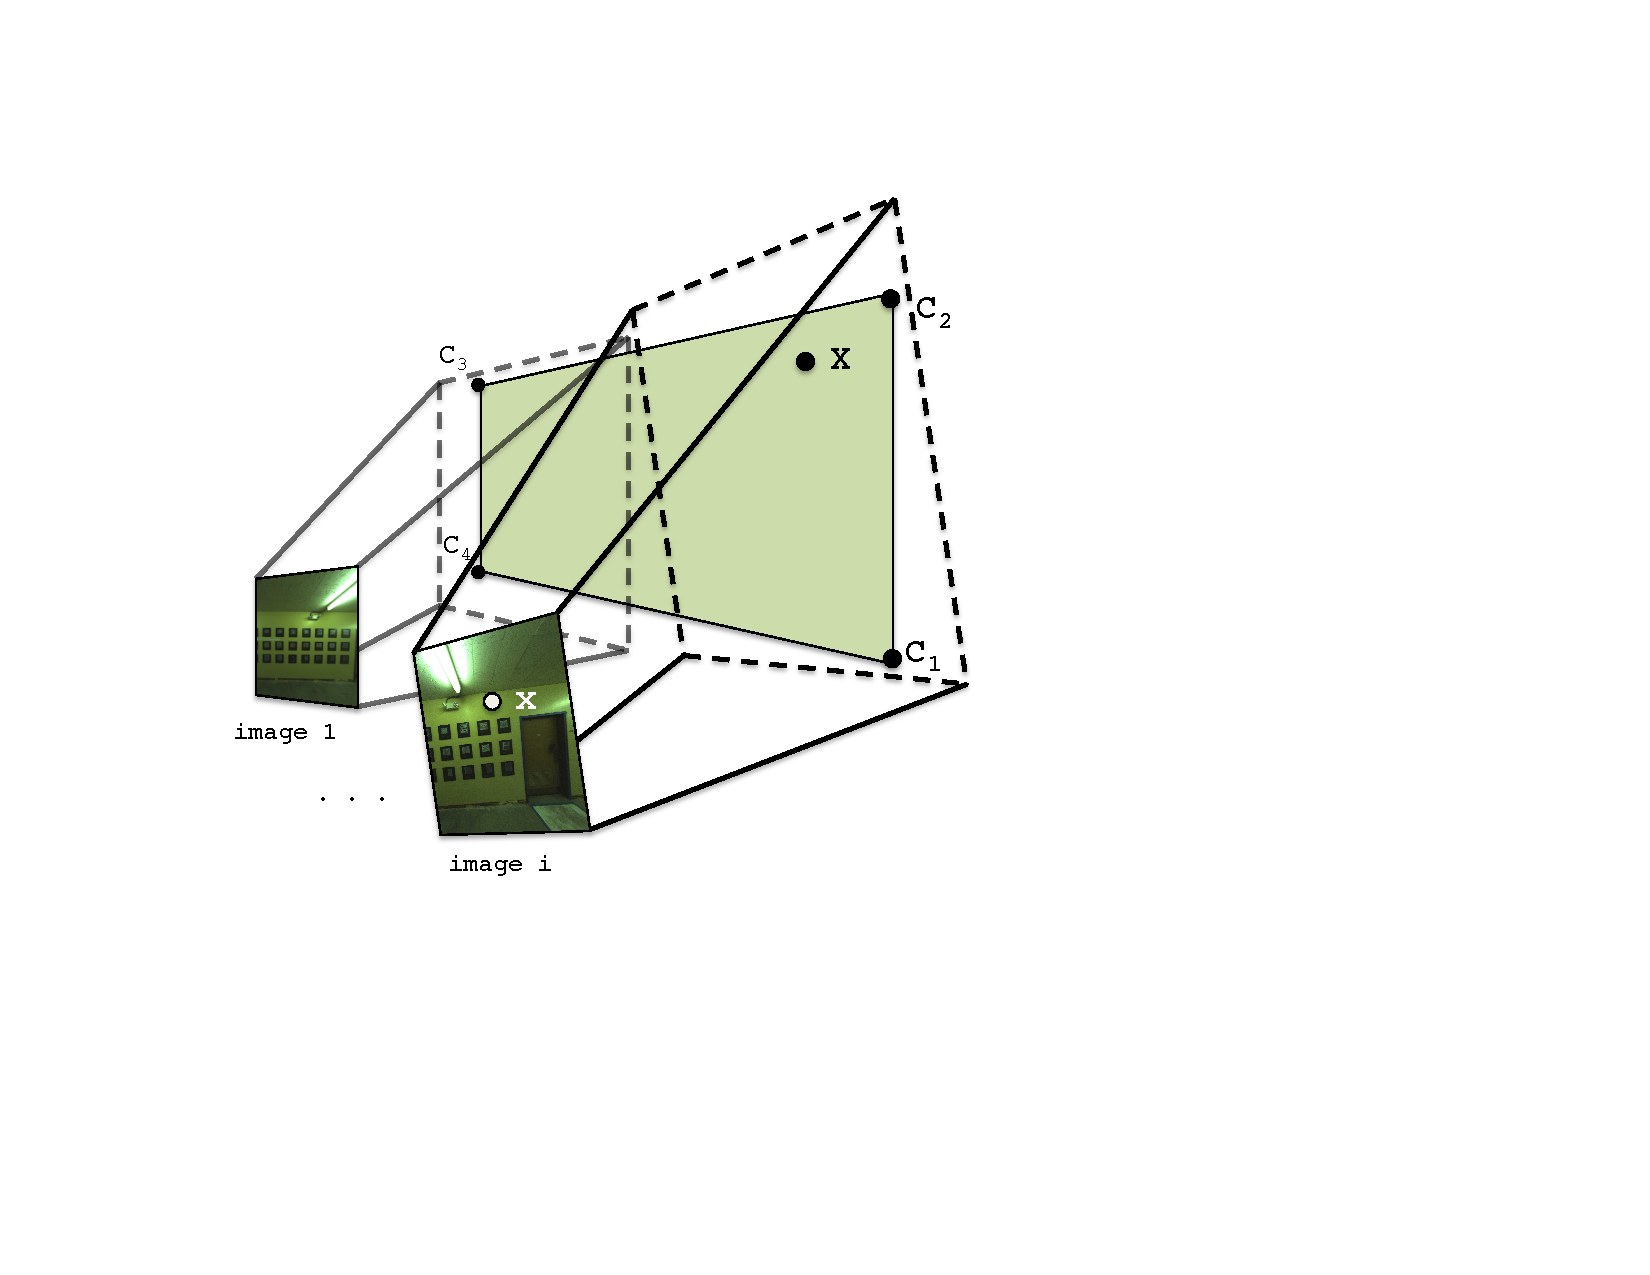
\includegraphics[height=2in]{Projection.pdf}
\caption{The plane is specified in 3D space by the four corners $C_1$ to $C_4$. Images are related to the plane through the camera matrices $P_{1..M}$. }
%\caption{The plane is specified in 3D space by the four corners $C_1$ to $C_4$. Images are related to the plane through the camera matrices $P_{1..M}$. For example, the 3D point X in the world coordinate system is related to the image point x shown in the figure as $x = P_i X$.}
\label{fig:projection}
\end{figure}


The geometry of the the texture mapping problem for indoor 3D modeling is shown in Figure 1. We are given a set of $M$ images. Each image has a camera matrix $P_i$ for $i=1..M$, which translates a point in the world coordinate system to a point in image $i$'s coordinates. A camera matrix $P_i$ is composed of the camera's intrinsic parameters, such as focal length and image center, as well as the extrinsic parameters which specify the rotation and translation of the camera center's position with respect to the world coordinates at the time that image $i$ was taken. These extrinsic parameters are determined by the localization hardware and algorithms as part of the indoor modeling system. A point $X$ on the plane can be related to its corresponding pixel $x$ in image $i$ through the following equation: 

\[
x=project(P_iX)
\]

where 
\[X = \begin{pmatrix} x \\ y \\ z \end{pmatrix} \textrm{ and } project(X) = \begin{pmatrix} x/z \\ y/z \end{pmatrix}
\]

We are also given a plane generated by the surface reconstruction system, which is to be texture mapped by these images. The plane is defined by four corner points $C_1$ to $C_4$ in world coordinates and a normal vector indicating the front facing side of the plane. The challenge is to texture the plane using these images, while eliminating any discontinuities or seams that would suggest that the plane was not composed of a single continuous image. 

\subsection{Best-Candidate Mapping}

\begin{figure}
\centering
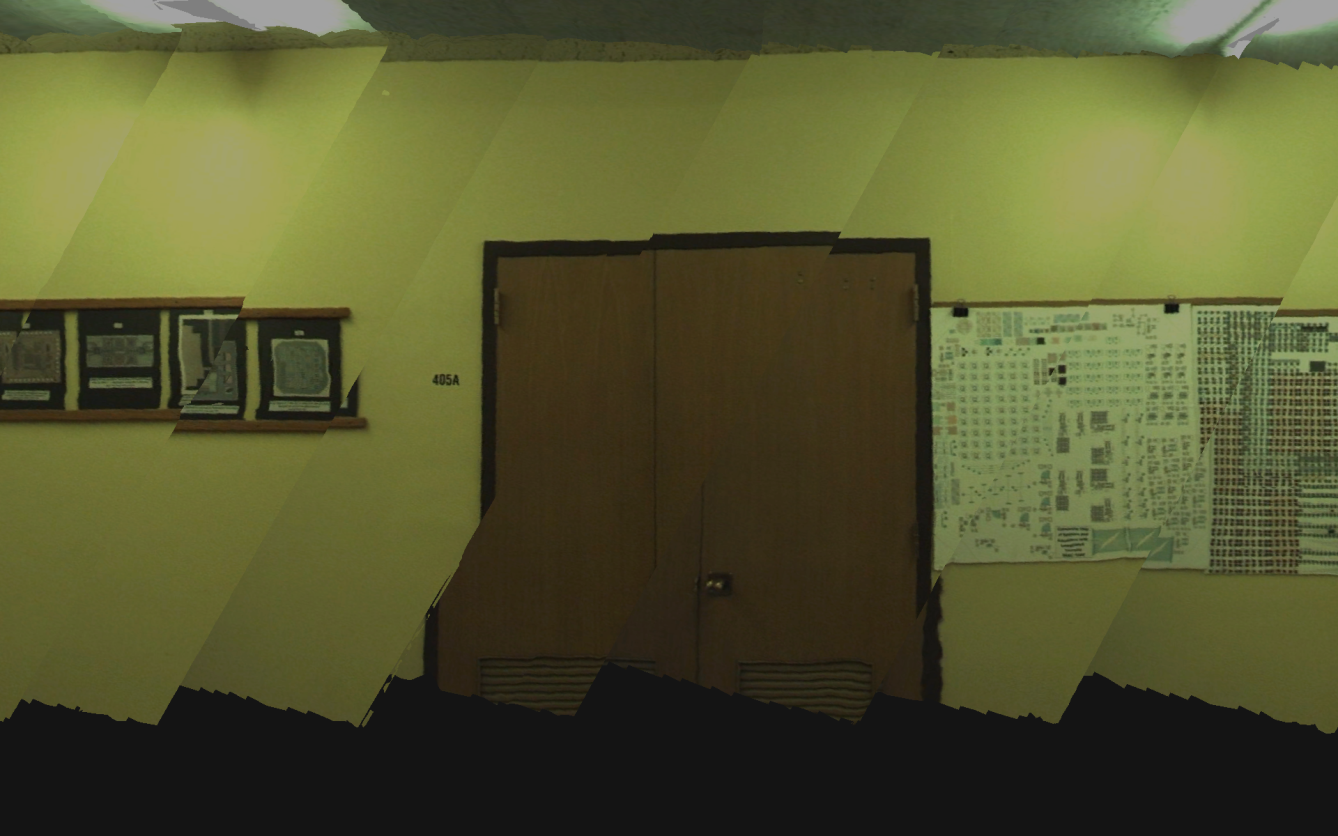
\includegraphics[height=1.5in]{naive.png}
\caption{The result of naive texture mapping based on the imprecise camera matrices estimated by the localization system.}
\label{fig:naive}
\end{figure}


Ignoring the fact that the camera matrices $P_{1..M}$ are inaccurate, one can texture map the plane simply by discretizing the plane into tiles or triangles and texturing each tile or triangle seperately. It makes sense to texture each tile or triangle by selecting a best candidate image. This is usually the nearest and/or most direct facing image to the tile or triangle. 

As Figure \ref{fig:naive} demonstrates, the best candidate mapping leads to significant misalignment between successive tiles. This suggests that while the errors in the localization system are quite low, they are not pixel accurate. For photorealistic texture mapping, either the camera matrices need to be refined such that the localization is pixel accurate, or image stitching techniques need to be applied to provide this illusion. The following are two existing techniques to solve this problem. 

\subsection{Image Mosaicing}

\begin{figure}
\centering
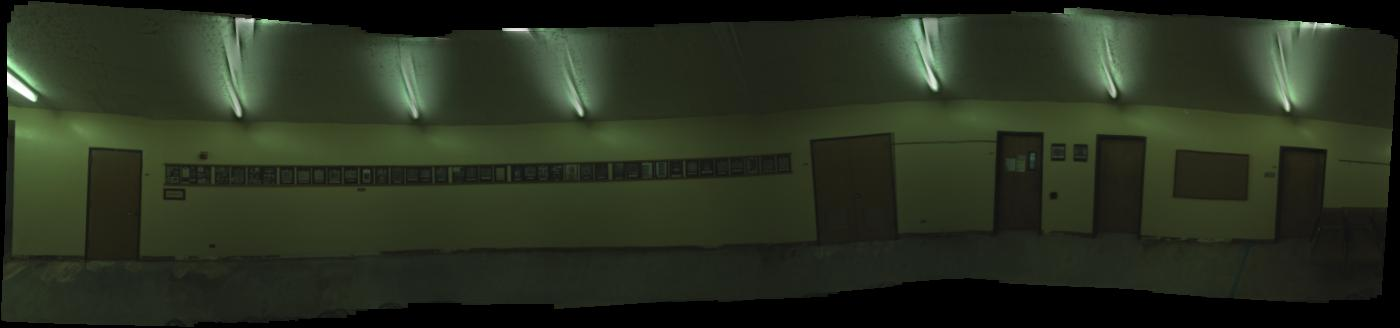
\includegraphics[width=4in]{panoMy.jpg}
\caption{Image mosaicing. }
\label{fig:mosaic}
\end{figure}


When images are taken of a plane from arbitrary overlapping positions, they are related by homography \cite{hz}. Thus, existing homography-based image mosaicing algorithms are applicable \cite{brown2007automatic}. However, errors can compound when long chains of images are mosaiced together using these approaches. For example, a pixel in the $n$th image in the chain must be translated into the first image's coordinates by multiplying by the $3\times3$ matrix $H_1 H_2 H_3 ... H_n$. Any error in one of these homography matrices is propagated to all further images until the chain is broken. For some chains of images this can happen almost immediately due to erroneous correspondence matches and the resulting image mosaic is grossly misshapen.

Figure \ref{fig:mosaic} shows the output of the AutoStitch software package which does homography-based image mosaicing. This plane is nearly a best-case scenerio with many features spread uniformly across it. Even so, the mosaicing produces errors that causes straight lines to appear as waves on the plane. This image was generated after careful hand tuning. Many planes that had fewer features simply failed. This led us to conclude that image mosaicing alone is not enough to reliably texture map our indoor 3D modeling dataset.

\subsection{Image-Based 3D Localization Refinement}

\begin{figure}
\centering

\includegraphics[width=3in]{Graph_crop.pdf}
\caption{Using the graph-based localization refinement algorithm from [11] suffers from the problem of compounding errors. }
\label{fig:graph}
\end{figure}

Another approach is to refine the camera matrices using image correspondences to guide the process. Each camera matrix has 6 degrees of freedom. Previous work attempted to refine the camera matrix by solving a non-linear optimization problem \cite{liu2010indoor}. This process is carried out at the same time as the laser based backpack localization and is therefore specific to the system in \cite{liu2010indoor,chen2010indoor}. Unfortunately, this approach suffers from a similar error propagation problem shown in Figure \ref{fig:graph}. In this work we also refine the placement of images using image correspondences. However, we do so in two dimensions on the plane where as this previous work did so over all 6 degrees of freedom. Refining in two dimensions on the plane is less flexible in that it cannot fix certain projection errors. Emperically we find that it avoids the error propagation problem.

\section{Our Approach}
\label{sec:approach}

Our approach can be summarized as follows. First we place all the images on the plane using the imprecise camera matrices given to us by the localization algorithm. This is done using the naive approach outlined in Section 2.1. This naive placement looks bad because the camera matrices are not pixel accurate. Our first challenge is to improve the placement of these images either by fixing the camera's localization in 3 dimeensions, or through 2 dimensional image processing techniques. We choose to use image processing techniques. SIFT matches are found between overlapping images. The imprecise localization means that matching SIFT features coming from two different images may not map to the same location on the plane. To fix this, we shift the images left, right, up, or down in such a way to maximize the agreement among images for each SIFT match. 

The next problem is image selection. The cameras on the backpack system produce far more images than are necessary to completely cover the plane. For example, a long hallway may have several hundereds of images when just 10 or 20 would suffice. We would prefer to use fewer images because this leads to fewer seams between images. However, we'd also like to make sure we are using good images that were taken perpendicular to the plane, for example, and whose seams fall in unimportant areas such as blank walls. In this section we outline two approaches to solving the image selection problem: a greedy heuristic solution that can work on any plane, and a dynamic programming formulation requires images overlap in a DAG structure. 

\subsection{Preprocessing}
As a starting point, we naively texture map the plane using the given imprecise camera matrices for each image in the set. This is done by discretizing the plane into an arbitrary density of pixels and projecting each pixel into the image plane using the estimated camera matrix $P_i$. We later intend to shift some of these projected images around on the plane and remove some others. Therefore, each image is stored intact in its own data structure so that it can later be merged with the other images on the plane. We use a Hough transform to rotate the projected images such that vertical lines are pointing directly upwards. This can be effective for indoor modeling, since many indoor scenes contain strong vertical lines from features such as doors, wall panels, or rectangular frames. 


\subsection{Localization Refinement}

The camera matrices generated by the localization algorithm are imprecise so the images are misaligned. To fix this, we choose to fix the locations in 2D. First we find corresponding points between all pairs of overlapping images using SIFT matches \cite{lowe1999object}. An illustration of this is given in Figure \ref{fig:matches}. The SIFT matches allow us to determine the correct $x$ and $y$ distances between two images on the plane. We already have an estimate of the $x$ and $y$ distances between the two images which was given by the localization algorithms. Soon we will compare the original estimates to the SIFT-based distances and use this to improve the quality of the image locations. 

\subsubsection{Robust SIFT Distances using RANSAC}

First we need to ensure that the SIFT-based distances are reliable. Since SIFT matches frequently include outliers, the RANSAC framework \cite{fischler1981random} is used for a robust estimate of the $x$ and $y$ distances between the two images. The RANSAC framework will attempt to build a consensus among the SIFT matches about what the true $x$ and $y$ distance is between the two images while ignoring the influence of outliers that may skew the results. The framework handles the consensus-building machinery, and only requires that two functions be specified: the fitting function and the distance function. These functions are called for random subsets of the SIFT matches until the best set of inliers is found. For this application, the fitting function simply finds the average distance between matches. If the matches are exactly correct and the image is frontal and planar then the distances for various SIFT feature matches should be the same. Our distance function for a pair of points is the difference between those points' SIFT match distance and the average distance computed by the fitting function. We specified a 10 pixel outlier threshold to the framework. This means that a SIFT match is labeled as an outlier if its $x$ and $y$ distance is not within 10 pixels of the average distance computed by the fitting function.

\subsubsection{Refining Image Positions using Least Squares}

There are a total of $M^{2}$ possible pairs of images, however we can only measure distances between images that overlap at SIFT feature points. Given these distances and the original image location estimates, we solve a least squares problem ($\textrm{min}_{\beta} ||\beta X - y||_2^2 $) to estimate the correct location of the images on the plane. The vector $\beta$ of unknowns are the correct $x$ and $y$ locations of each image on the plane from $1 \dots M$. Finding the correct $x$ and $y$ locations are independent from one another so we will only consider the $x$ locations:

% Draw least squares problem here. 

\[\beta =
 \begin{pmatrix}
  x_1, & x_2, & x_3, & \cdots & x_{M-1}, & x_M
 \end{pmatrix}
\]

The matrix $X$ is constructed with one row for each pair of images with measured distances produced by the SIFT matching stage. A row in the matrix has a $-1$ and $1$ in the columns corresponding to the two images in the pair. For example, the matrix below indicates that we generated a SIFT-based distance between images 1 and 2, images 1 and 3, images 2 and 3, etc. 

\[
 X =
 \begin{pmatrix}
  -1 & 1 & 0 & \cdots & 0 & 0\\
  -1 & 0 & 1 & \cdots & 0 & 0\\
   0 & -1 & 1 & \cdots & 0 & 0\\
  \vdots  & \vdots & \vdots & \ddots & \vdots  & \vdots\\
  0 & 0 & 0 & \cdots & 1 & 0 \\ 
  0 & 0 & 0 & \cdots & -1 & 1 \\ 
  1 & 0 & 0 & \cdots & 0 & 0 \\ 
 \end{pmatrix}
\]

If only relative distances between images are included then there is no way to determine the absolute location of any of the images and the matrix becomes rank deficient. To fix this we choose the first image to serve as the anchor for the rest, meaning all the absolute distances are based on its original location. This is done by adding a row with a $1$ in the first column and the rest zeros. 

Finally, the observation vector $y$ is constructed using the SIFT-based distances generated earlier in the matching stage. The distances are denoted as $d_1 \dots d_N$ for $N$ SIFT-based distances. The last element in the observation vector is the original location of the first image determined by the localization algorithm. 

\[
y^T = 
 \begin{pmatrix}
  d_{1,2}, & d_{1,3}, & d_{2,3}, & \hdots & d_{N-2,N-1}, & d_{N-1,N}, &  x_1
 \end{pmatrix}
\]

The $\beta$ that minimizes  $||\beta X - y||_2^2$ tells us a set of image locations on the plane that best honors all the SIFT-based distance measurements between images. A similar problem is solved for the $y$ dimension. In practice there are often cases where there is a break in the chain of images, meaning that no SIFT matches were found between one segment of the plane and another. In this case we add rows to the $X$ matrix and observations to the $y$ vector that contain the original $x$ and $y$ distance estimates generated by the localization algorithm. Another way to do this is to add rows for all neighboring pairs of images and solve a weighted least squares problem where the SIFT distances are given a higher weight i.e. 1, and the distances generated by the localization algorithm are given a smaller weight i.e. 0.01. 



%Given these corresponding points, we can align the neighboring projected images by setting the pixel location of the right projected image based on the pixel location of the left projected image and the average distance between the SIFT matches. Note that we are solving for two variables: the x and y coordinates of the right projected image's pixel location on the plane.  Intuitively speaking, we are taking pairs of images and sliding the right image horizontally and vertically until the corresponding points overlap. If no matches can be found between neighboring images, they are left in their originally estimated locations. 
%
%\begin{figure}
%\begin{lstlisting}
%% RANSAC fitting function
%function shift = fit_shift(x1, x2)
%    % Average distance between matches
%    shift = mean(x1-x2,2); 	
%
%% RANSAC distance function
%function [inliers, shift] = 
%         shiftdist(shift, x1, x2, t);
%    % Find the shift error for each match
%    shiftmat = repmat(shift,1,size(x2,2));
%    err = sum(abs(x1-(x2+shiftmat)));
%    % Inliers are those with error less than t
%    inliers = find(abs(err) < t);
%
%\end{lstlisting}
%\caption{Fitting function and distance function for RANSAC.}
%\end{figure}



\subsection{Image Selection}

The backpack system produces images at a much faster rate than is necessary to fully texture map all surfaces. Many of these images can be discarded because the range they cover is also covered by other images in the set. In fact, our system discards images as a preprocessing step that are either not directly facing the plane or are beyond a certain threshold distance from each plane. Beyond this, it can be advantageous to throw away redundant images at this stage because fewer images generate fewer seams and therefore fewer potential visual artifacts from misalignment. We describe two methods for image selection. The first is a greedy heuristic that makes no assumption about the plane or the images. The second method assumes that the images overlap in a DAG structure and employs dynamic programming to minimize a specific cost associated with a selection of images. 

\subsubsection{Greedy Heuristic}

We begin with an empty plane and a set of $M$ images. The image that covers the largest number of pixels on the plane is chosen and copied to the plane. The pixels covered by that image are then considered to be covered. Next, the image that covers the largest number of uncovered pixels is chosen. It is copied to the plane as well. If it overlaps with any covered pixels then the image is blended according to the process described in Section 4.1.2. This process continues until the plane is completely covered. 

\subsubsection{Cost Functions}

The greedy algorithm will cover the plane, if possible, and will tend toward using fewer images. However, the solution is not optimal with respect to any image-based cost. We may be interested in covering the plane while minimizing the sum of squared pixel differences of the blended seam regions. This would encourage seams to be placed either in featureless areas, such as blank walls, or in areas in which the images are very well aligned. Another possible cost function is edge energy, i.e. the sum of the smoothed gradient of the blended seam regions. This would encourage seams to be placed in featureless areas even more than the sum of squared pixel difference cost function. 


\subsubsection{Dynamic Programming}

\begin{figure}
\centering
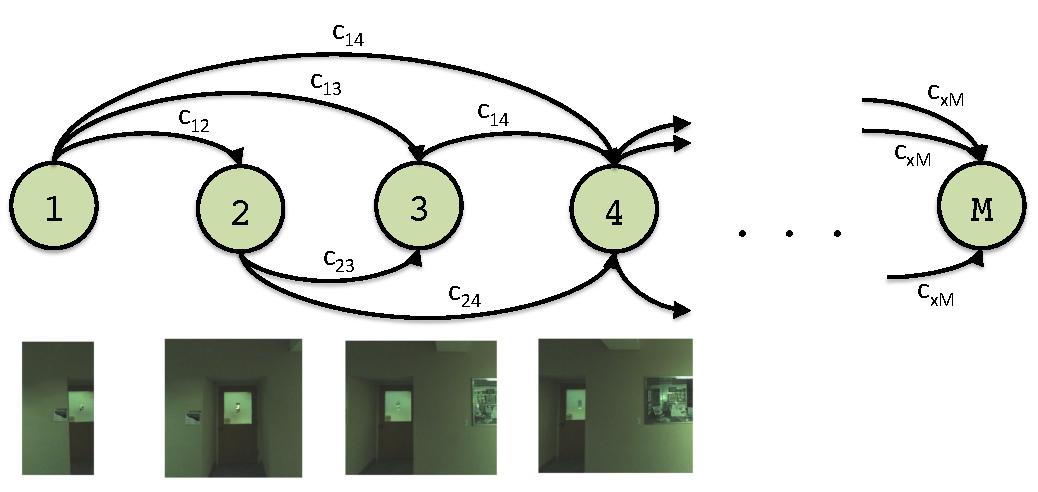
\includegraphics[width=3in]{DynProg.pdf}
\caption{Image Selection is done by constructing a graph of sorted images. Then we solve a shortest path problem where the edge weights represent the cost of a seam between two overlapping images.}
\label{fig:DynProg}
\end{figure}

In the general case, finding the optimal subset of images with regard to the cost functions appears to have exponential complexity in the number of images. For this reason, we did not attempt this approach to image selection. However, if the images overlap only in one direction, as they do in long hallways, we can construct a DAG from the overlapping images and solve a simple shortest path problem to find an optimal subset of images with regard to the cost functions.

Figure \ref{fig:DynProg} demonstrates the construction of a DAG from overlapping images of a long hallway. Images are sorted by location (e.g. left to right) and become nodes in a graph. Edges are placed in the graph between images that overlap. The weights of these edges are determined by a cost function, such as image energy, or the sum of squared pixel differences between the two images in the seam region. Next, we solve a shortest path problem from the first node in the graph to the last node. This provides a set of images that completely covers the plane, but minimizes the cost of the seams produced. Note that this only works when all the images completely cover one dimension. In this case the vertical dimension of the plane is covered by all images. 

\subsection{Blending}

The steps above eliminate visual artifacts from misalignment, but there still are obvious discontinuities in brightness between images resulting from differences in lighting. This problem has been successfully addressed in previous work using an alpha blending technique in which the pixel intensities in overlapping images are blended proportional to the pixel's location in the image \cite{liu2010indoor}. We use a similar technique to improve the visual quality of our results. In the small area where images overlap, there is a linear weighting function in the horizontal direction that interpolates between the left image and the right, providing a gradual transition between images. The final location corrected, subsampled, and blended image is shown in Figure \ref{fig:window4}.

\section{Results}
\label{sec:results}

\section{Conclusions and Future Work}
\label{sec:results}


\bibliographystyle{IEEEbib}
\small
\bibliography{strings,refs}




\message{ !name(isvc_submission.tex) !offset(-5) }

\end{document}
